Dịch vụ máy chủ mở (Open Host Service) là nhà cung cấp trong mô hình khách hàng - nhà cung cấp, dịch vụ máy chủ mở hiển thị một API công khai cho các bối cảnh bị giới hạn khác sử dụng chức năng của nhà cung cấp.

Trong bản đồ bối cảnh, dịch vụ máy chủ mở được ký hiệu là OHS.

% Vẽ lại bản đồ tiếng Việt

% Vẽ lại bản đồ tiếng Việt

% Vẽ lại bản đồ tiếng Việt

% Vẽ lại bản đồ tiếng Việt

% Vẽ lại bản đồ tiếng Việt

% Vẽ lại bản đồ tiếng Việt

% Vẽ lại bản đồ tiếng Việt

% Vẽ lại bản đồ tiếng Việt

% Từ bản đồ lấy vi dụ cho các mô hình

% Từ bản đồ lấy vi dụ cho các mô hình

% Từ bản đồ lấy vi dụ cho các mô hình

% Từ bản đồ lấy vi dụ cho các mô hình

% Từ bản đồ lấy vi dụ cho các mô hình

% Từ bản đồ lấy vi dụ cho các mô hình

% Từ bản đồ lấy vi dụ cho các mô hình

% Từ bản đồ lấy vi dụ cho các mô hình

% Từ bản đồ lấy vi dụ cho các mô hình

% Từ bản đồ lấy vi dụ cho các mô hình

\begin{example} Trong miền vấn đề ngân hàng, thẻ tín dụng và khoản vay mua nhà không có mối quan hệ.

\begin{figure}[H]

\centering

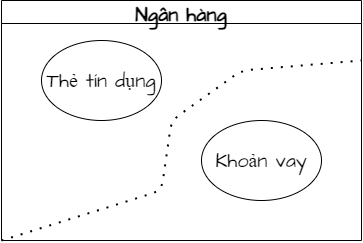
\includegraphics[scale = 0.5]{pictures/mo_hinh_rieng_biet_separate_ways/main.drawio.png}

\caption{Ví dụ mô hình riêng biệt (Separate Ways)}

\end{figure}

\end{example}

